%% ============================================================================
%% ============================================================================
\section{Robustness and the Specificity Panel}
\label{sec:sensitivity}

The headline result uses the aggregator composite, the only feed covering every hour of
the window, corroborated by the fiat-settled venue that carries USDC. Kraken's
USDC/USD close breaches the \$0.92 floor in 9 of 240 hours and its VWAP series
breaches it in 10 (Table~\ref{tab:firing}). The hourly low breaches it in 12, but the
three extra hours rest on one print: the \$0.874 low is a 3,373.52-USDC trade worth
\$2,948, about $0.01\%$ of that hour's traded volume. Binance corroborates depth only
(Section~\ref{sec:setting}).

% Source: results/phi_denominator_sensitivity.json --
%   Sentence 1: feed_trough_only_at_phi_0.08 (added to
%     phi_denominator_sensitivity.py and regenerated; restricted to the four genuinely
%     distinct price feeds, excluding composite_second_lowest which is a second print
%     within the composite feed, not a fifth feed): s_nf0_min=0.1919 (kraken_close_min),
%     s_nf0_max=0.3513 (composite_min_headline).
%   Sentence 2: full grid[] range across all 3 phi conventions x 5 trough readings
%     (min/max of grid[].s_nf0): 0.1667 (phi=0.0825, kraken_close_min) to 0.3643
%     (phi=0.0784, composite_min_headline). Pinned by
%     tests/test_phi_denominator_sensitivity.py::test_feed_trough_only_at_phi_08_excludes_second_composite_print
%     and ::test_broader_grid_range_includes_non_feed_cells.
At $\phi=0.08$, restricted to the four price feeds' own troughs (composite, Kraken close,
Kraken VWAP, and Binance/USDT-deflated), the non-fundamental share $s_{\mathrm{nf}}(0)$ ranges from
$19.2\%$ (Kraken close) to $35.1\%$ (composite).
A broader sensitivity range should not be conflated with it. That range runs over the
full grid of three $\phi$ conventions (0.0784, 0.08, 0.0825) and all five
trough readings, which add the composite feed's second-lowest print
($\$0.8949$) to the four feed troughs above.
It spans $16.7\%$ to $36.4\%$.

Kraken's close series is autocorrelated (lag-1 $=0.945$), so its 240 readings carry an
effective sample size of $6.7$, and the 9 breaching hours measure a duration rather
than 9 statistically independent observations.

The impairment loss is fixed in dollars while redemptions shrink the reserve base, so
$\phi$ moves inversely with it. At the composite trough $\phi$ is $0.079$, below the headline
$0.08$, so the floor rises to \$0.921. Supply is observed only daily. The two
snapshots bracketing the trough admit an interpolation band $\phi\in[0.078,0.081]$, over
which the count of breaching hours ranges from 9 to 11. Computed hour by hour, $\phi$
reaches its highest value in the last hour of the window, and that maximum is a censoring
artifact.
At that hour the coin trades at \$1.004 and $q^{\star}=-0.044$, so the bound is vacuous
there and the maximum falls on the last observed day. We report the band as a bound on
how far the correction can move $\phi$. Daily supply data cannot resolve a finer
measurement.

\begin{table}[t]
\centering
\caption{Breaching hours against the \$0.92 floor, over each series' own observed window,
for the feeds that cover the trough: the composite for USDC, DAI, and USDT, and
Kraken's close, VWAP, and low for USDC. Binance is excluded because its series begins after
the trough.}
\label{tab:firing}
\small
\checkwidth{\small% Source: results/trough_corroboration.json --
%   firing_report.series.{composite, kraken_usdc_close, kraken_usdc_vwap,
%   kraken_usdc_low}.{firing_count, n_hours_observed} (9/212, 9/240, 10/240, 12/240);
%   results/impossibility_window.json coins.{DAI,USDT}.{breaching_hours,
%   hours_observed} (2/214, 0/213). Replaces the old Figure 1 lower strip,
%   deleted along with that figure.
%   The Kraken-low single-trade caveat (trough_corroboration.json's
%   kraken_low_convention_note) is not reproduced here -- see write_tab_firing
%   docstring; that caveat now lives in body prose.
\begin{tabular}{@{}lc@{}}
\toprule
Feed & Breaches \\
\midrule
Composite (USDC) & 9/212 \\
Kraken close (USDC) & 9/240 \\
Kraken VWAP (USDC) & 10/240 \\
Kraken low (USDC) & 12/240 \\
DAI (composite) & 2/214 \\
USDT (composite) & 0/213 \\
\bottomrule
\end{tabular}
}
% Source: results/trough_corroboration.json --
%   firing_report.series.{composite, kraken_usdc_close, kraken_usdc_vwap,
%   kraken_usdc_low}.{firing_count, n_hours_observed} (9/212, 9/240, 10/240, 12/240);
%   results/impossibility_window.json coins.{DAI,USDT}.{breaching_hours,
%   hours_observed} (2/214, 0/213). Replaces the old Figure 1 lower strip,
%   deleted along with that figure.
%   The Kraken-low single-trade caveat (trough_corroboration.json's
%   kraken_low_convention_note) is not reproduced here -- see write_tab_firing
%   docstring; that caveat now lives in body prose.
\begin{tabular}{@{}lc@{}}
\toprule
Feed & Breaches \\
\midrule
Composite (USDC) & 9/212 \\
Kraken close (USDC) & 9/240 \\
Kraken VWAP (USDC) & 10/240 \\
Kraken low (USDC) & 12/240 \\
DAI (composite) & 2/214 \\
USDT (composite) & 0/213 \\
\bottomrule
\end{tabular}

\end{table}

\begin{table}[t]
\centering
\caption{Specificity panel across three candidate episodes. USDC (2023) is the panel's one
true positive, with the floor breached under all sixteen combinations of four price
conventions and four $\phi$ readings: the three disclosed denominators of
Section~\ref{sec:ident} and the dilution-adjusted $\phi=0.079$. The row shown is
$\phi=0.08$ against the composite trough, and $q^{\star}$ is undefined where $\phi=0$.}
\label{tab:panel}
\small
\setlength{\tabcolsep}{2pt}
\checkwidth{\small\setlength{\tabcolsep}{2pt}\input{tables/tab_panel}}
\input{tables/tab_panel}
\end{table}

\paragraph{Why only one episode meets the preconditions.}
The estimator requires three preconditions. First~(i), $\phi$ must be publicly quantified
while the exposure is unresolved. Second~(ii), the price must fall more than $1\%$ below
par while that disclosure is live. Third~(iii), the fundamental channel must be
reserve-only, so that $1-\phi$ is the floor. We screened seven candidates: BUSD, Tether~(2022),
DAI~(2020), USDR, USDP, GUSD, and TUSD. \emph{None satisfies all three.} Each candidate
fails in one of two ways: no disclosed impairment or a loss measured under a different
valuation model (Appendix~\ref{app:excl}). Issuers with a material impairment did not
disclose its size in any of the seven screened cases, so one qualifying episode is a property of the
disclosure record.

Tether's episode is assessed under precondition~(i): $\phi$ publicly quantified while the
exposure was unresolved. The NYAG's 25~April 2019 statement quantified Tether's exposure
and Tether contested the characterization. The statement implies $\phi\in[0.259,0.332]$.
The deepest post-disclosure Kraken USDT/USD print, \$0.9551 on 26~April 2019, is 21.4 to
28.8 cents above every worst-case floor. USDT, Terra episode (May 2022), is the degenerate control, with $\phi=0$, a floor at par, and $q^{\star}$ undefined. Paxos's USDP is a timing control and is not
in the panel. Its only quantified exposure was \$250M at Signature Bank. Paxos disclosed
it 80 minutes after the joint statement~\cite{fedtreasfdic2023pressrelease} had already
guaranteed the deposits Paxos described.

\begin{figure}[t]
\centering
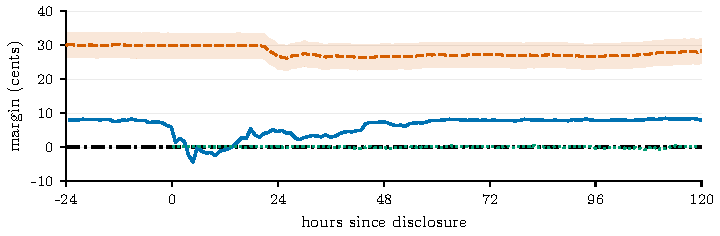
\includegraphics[width=\textwidth]{figs/fig_margin_paths.pdf}
\caption{Each episode's margin, price minus its own floor in cents, from 24~hours before
to 120~hours after its own quantification. Zero is the floor:
USDC~2023 (solid) breaches it, Tether~2019 (dashed, with its regulator-quantified floor
range shown as a band) and USDT, Terra episode (May 2022) (dotted), do not.
The Terra floor is par because $\phi=0$.}
\label{fig:margin_paths}
\end{figure}

The panel holds one true positive, one episode on which the bound returns no verdict, and
one degenerate control (Figure~\ref{fig:margin_paths}). USDC in 2023 is the true
positive: the floor is breached under all sixteen combinations of $\phi$ and price convention, and the trough requires an unremediated-loss probability of
$1.20$--$1.61$. Tether in 2019 is regulator-quantified and
issuer-contested, with $\phi\in[0.259,0.332]$, a trough $21.4$--$28.8$ cents above its
floor, and $q^{\star}\in[0.135,0.174]$. The degenerate control is USDT, Terra episode (May
2022), with $\phi=0$, not counted. We exclude the Reserve Primary Fund of 2008 because its
published figure is a NAV rather than a market price. The Tether row's $\phi$ comes from a
regulator, who quantified the exposure publicly at the time, and not from Tether's own
disclosure. Because the quantification is the regulator's and Tether contests it, the
panel contains no validated true negative under precondition~(i), $\phi$ publicly
quantified while the exposure was unresolved. The specificity of the bound is unmeasured.
